To test the surrogate model assisted (1+1)-ES with various degrees of surrogate model exploitation under $(\mu/\mu,\lambda)$ preselection, we use three sets of test problems and, for each test problem, experiment with a range of parameters over dimension $n$ = 2, 4, 8, and 16. The test problems used are namely, sphere functions $f(x) = (x^Tx)^{\alpha/2}$ for $\alpha \in [0.25,4]$, $f(x) = \sum_{i=1}^{n-1}[\beta (x_{i+1} - x_i^2)^2 + (1-x_i)^2]$ referred to as the quartic function for $\beta \in [1,5]$, and the ellipsoid functions $f(x)=x^TAx$, $A=\text{diag}(\beta,1,...,1)$ for $\gamma \in [10^{-2},10^2] $. The latter two problems test the ability of the algorithm to handle ill-conditioned problems. The quartic function becomes the Rosenbrock function when $\beta = 100$ with the condition number of the Hessian at the optimizer exceeds 3,500. We start with $\beta$=1 and end with $\beta$=5 where the condition number of the Hessian at the optimizer is 49.0 and $\color{red}{?}$ respectively. When $\gamma \ll$, the ellipsoid function becomes the cigar function, whereas the discus function is obtained as $\gamma \gg 1$. The optimal value of all the test problems is zero. 

For each test problem, we choose 11 different values for each range (of $\alpha,\beta$, and $\gamma$) in the three test functions and conduct 51 runs for both the (1+1)-ES without surrogate model assistance and the surrogate model assisted (1+1)-ES with $(\mu/\mu,\lambda)$ preselction ($\lambda \in \{1,10,20,40\}$ and $\mu = \lceil \lambda/4 \rceil$). The Gaussian process surrogate is used for surrogate modelling purposes. For simplicity, we use the same  setting from Kayhani and Arnold \cite{} where the kernel is squared exponential kernel and the length scale parameter of the kernel being $8 \sigma \sqrt{n}$ $\sigma$ where $\sigma$ is the step size parameter in the evolutionary strategy. The training set contains the most recently evaluated $20+2n$ candidate solutions. That is, the algorithm starts with a (1+1)-ES in the first $20+2n$ iterations and the surrogate model is used to assist the (1+1)-ES once the it is in place (after the first $20+2n$ iterations). All runs are initialized from sampling a Gaussian distribution with mean zero and unit covariance matrix (except in the sphere function that the initial candidate solution is sampled from a unit covariance matrix mutiplied by a factor of 1000 for comparison purposes). All initial step sizes are set to $\sigma=1$ and all runs terminate when the objective function value of a candidate solution is below $10^{-8}$. 

\begin{center}
\begin{figure*}
    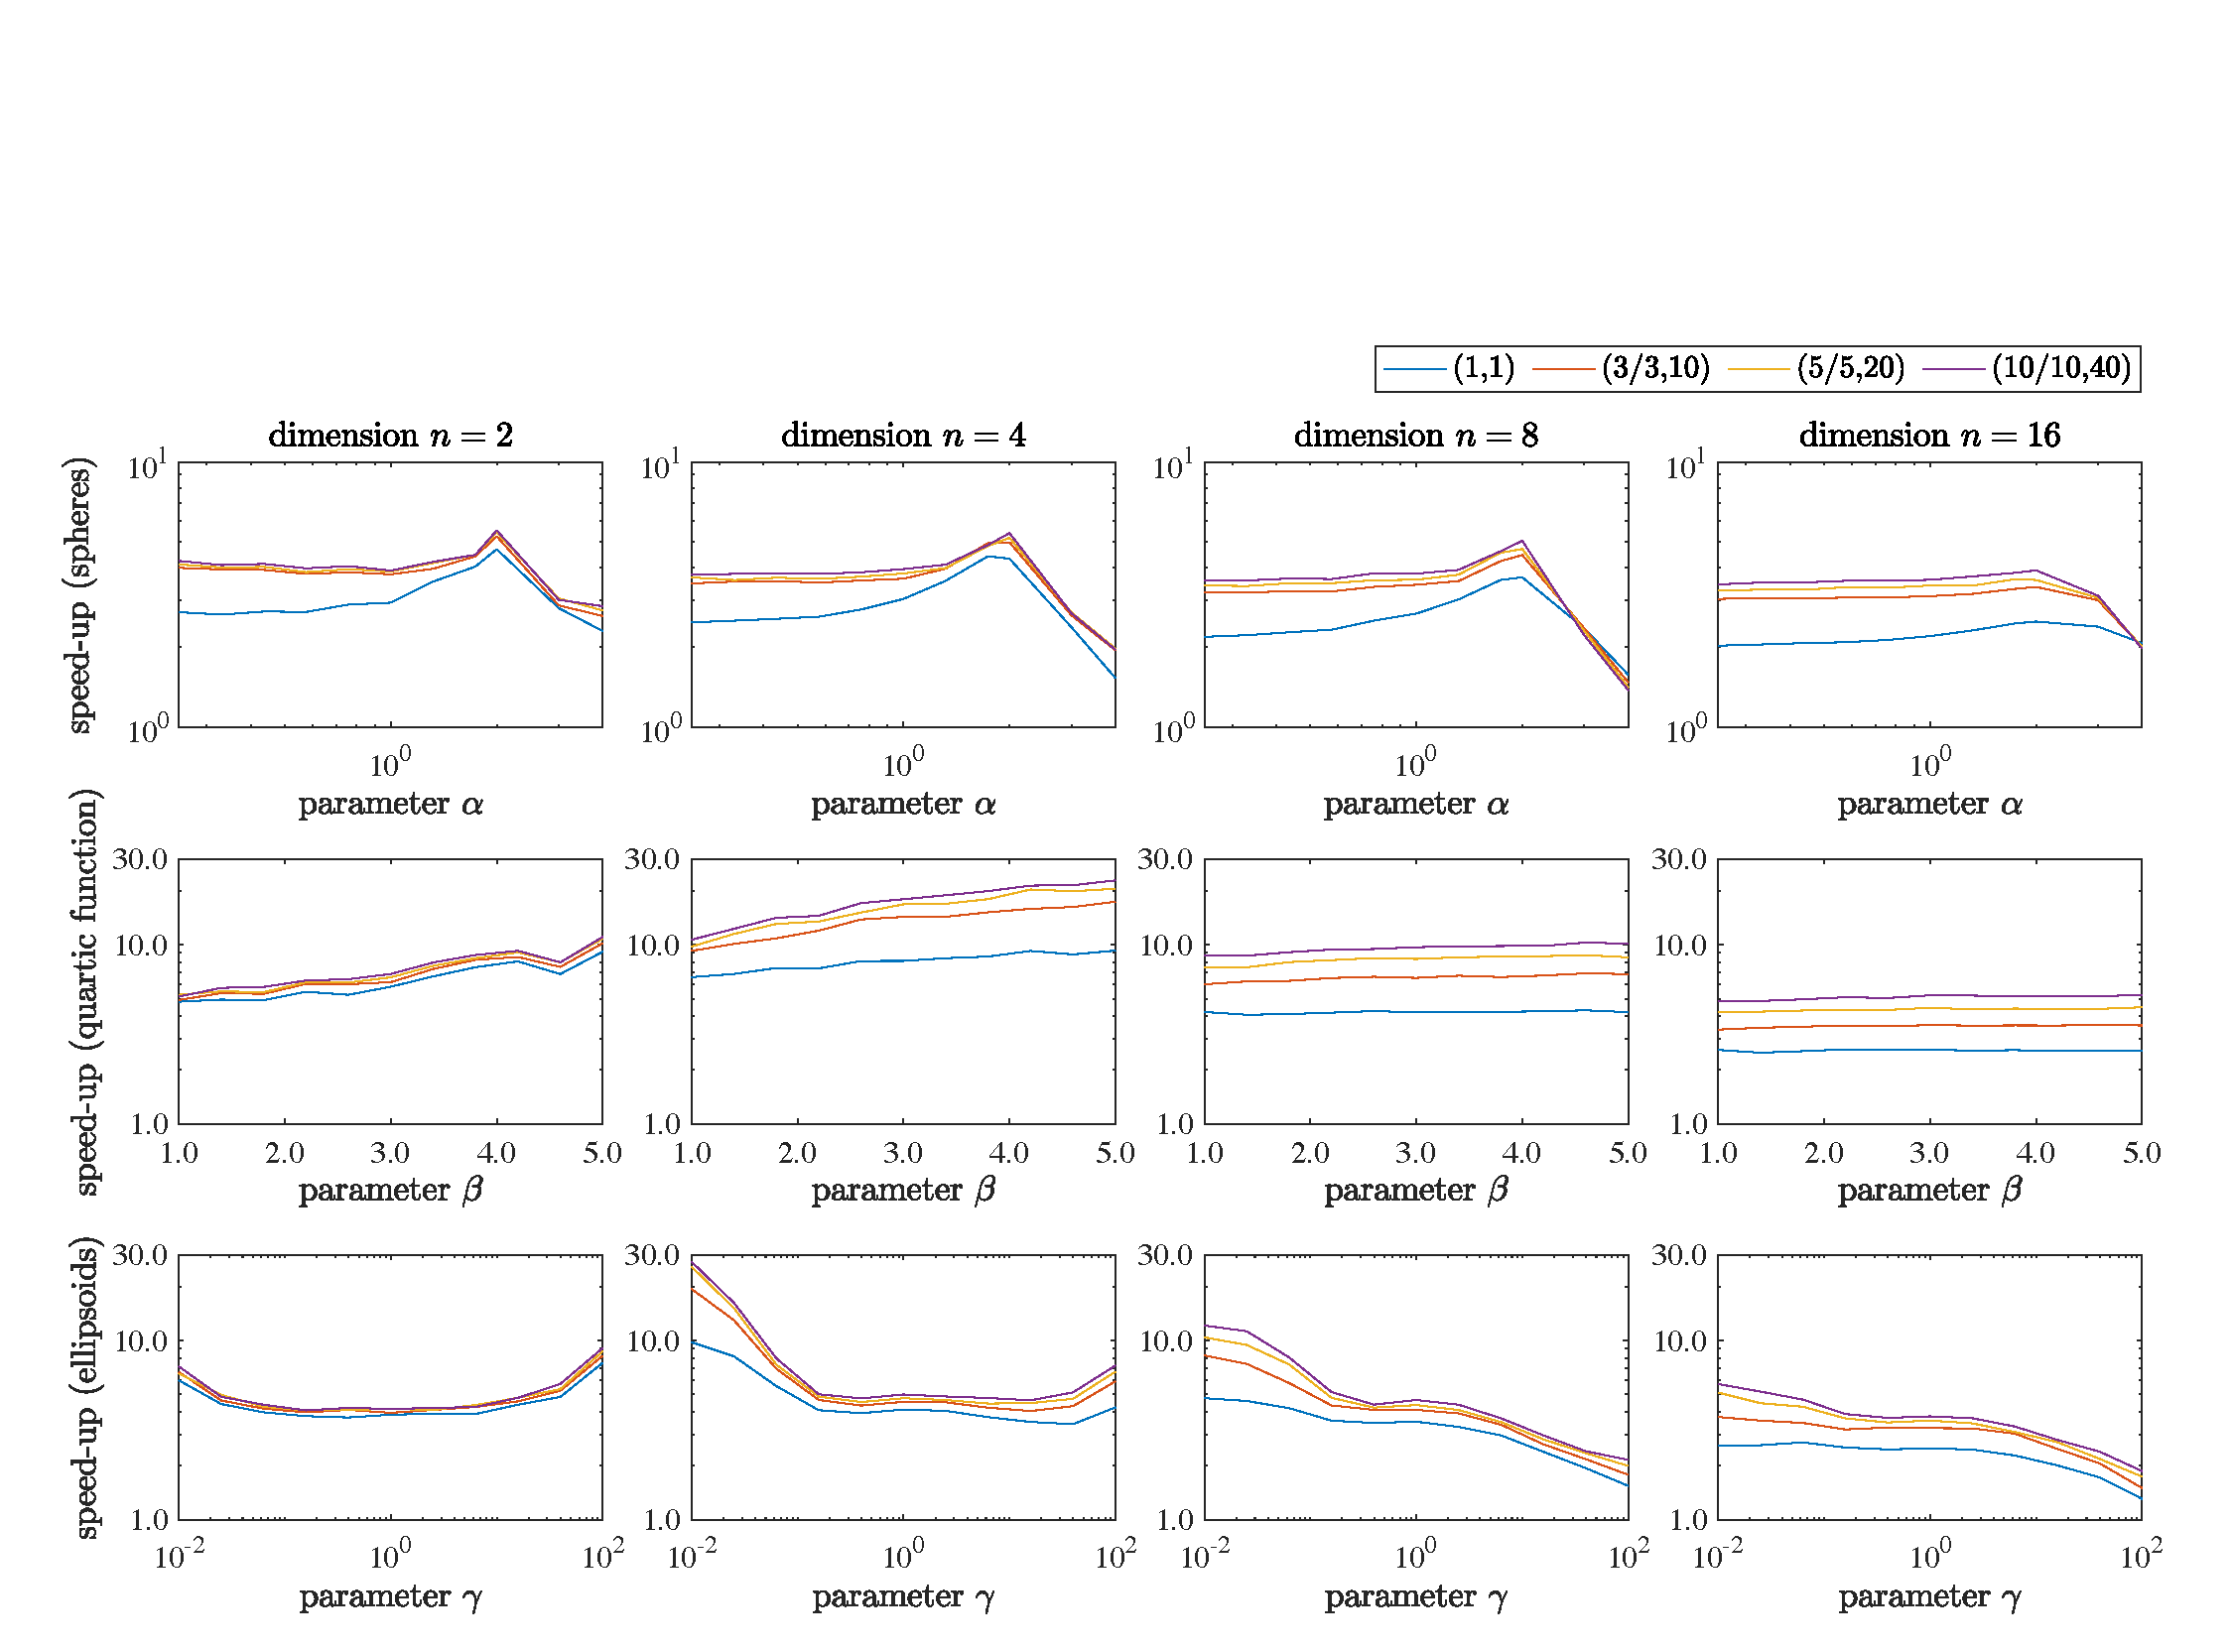
\includegraphics[width=1 \linewidth]{speed-up_legend-top.pdf}
    \caption{Speed-ups observed in median runs. From top to bottom, each row represents the speed-up observed in the sphere function, quartic function, and ellipsoids function respectively. Whereas each column illustrates a test problem in different dimension and from left to right has dimension $n=2,4,8,16$. Each individual plot shows the speed-ups of surrogate model assisted (1+)-ES with $(\mu/\mu,\lambda)$ preselection where $\lambda=1,10,20,40$ and $\mu=\lceil \lambda /4\rceil$.}
    \label{fig:speed-ups}
\end{figure*}
\end{center}

The speed-ups reported in Fig. \ref{fig:speed-ups} are obtained using the median-run results (with the base of (1+1)-ES without surrogate model assistance). Even if in the quartic functions and ellipsoids, the speed-ups for surrogate model assisted (1+1)-ES decrease as the dimension of the problem becomes larger. The overall speed-up achieved is between 2 and 5 in spheres 3 and 20 in quartic functions, and 2 to 10 in ellipsoids. On the whole, the surrogate model assisted (1+1)-ES with more model exploitation (a large $\lambda$ in $(\mu/\mu,\lambda)$ preselction) has larger values of speed-ups. When $n \geq 4$, the speed-ups achieved for surrogate model assisted (1+1)-ES ((1,1) preselection) doubled after the deployment of a $(10/10,40)$ preselection. Similarly, in the case of spheres and ellipsoids, the speed-ups  also increase by 30\% to 60\% with a preselection using $\lambda=40$ as opposed to that of a $(1,1)$. However, there is a decreasing trend in the speed-ups in spheres ($\alpha \geq 2$ for all dimensions) and the ellipsoids ($\gamma \geq 1$ for $n\geq 8$) as the parameter of the problem increases. This is potentially resulted from a less accurate Gaussian process surrogate model given a possible too large training size relative to the number of objective function evaluations used to solve the problem (the surrogate model is updated too slowly). With the example of dimension n=8, the number of objective function evaluations needed to solve the sphere functions in median run for (1+1)-ES is 4373 when $\alpha=0.25$ but 709 when $\alpha=4$. Similarly, the number for (1+1)-ES to solve the ellipsoids when n=8 for $\gamma = 10^{-2}$ and $10^2$ are 9287 and 1278 respectively. 

